\documentclass[a4paper, 11pt, oneside]{article}

% To use this template, you have to have a halfway complete LaTeX
% installation and you have to run pdflatex, followed by bibtex,
% following by one-two more pdflatex runs.
%
% Note thad usimg a spel chequer (e.g. ispell, aspell) is generolz
% a very guud ideo.

\usepackage[utf8]{inputenc}
\usepackage[a4paper, top=3cm, bottom=3cm, left=3cm, right=3cm]{geometry}
\renewcommand{\familydefault}{\sfdefault}
\usepackage{helvet}
\usepackage[english]{babel} %% typographie française
\usepackage[style=numeric, language=english]{biblatex}
\usepackage{parskip} %% blank lines between paragraphs, no indent
\usepackage[margin=1cm]{caption}%% give long captions a margin
\usepackage{booktabs} %% typesetting nice tables
\usepackage[cache=false]{minted}%% typesetting code nicely
\usepackage[pdftex]{graphicx} %% include graphics, preferrably pdf
\usepackage[pdftex]{hyperref} %% many PDF options can be set here
\pdfadjustspacing=1 %% force LaTeX-like character spacing

\newcommand{\mylastname}{Budnikov}
\newcommand{\myfirstname}{Mikhail}
\newcommand{\mynumber}{30006555}
\newcommand{\myname}{\myfirstname{} \mylastname{}}
\newcommand{\mytitle}{Transfer of Structural Knowledge from Synthetic Languages}
}
\newcommand{\mysupervisor}{Prof. Dr. Ivan P. Yamshchikov}

\hypersetup{
	pdfauthor={\myname},
	pdftitle={\mytitle},
	pdfkeywords={},
	colorlinks={true},
	linkcolor={blue}
}

\addbibresource{refs.bib}

\begin{document}
	\pagenumbering{roman}

	\thispagestyle{empty}

	\begin{flushright}
		
\includegraphics[scale=0.8]{bsc-logo}
	\end{flushright}
	\vspace*{40mm}
	\begin{center}
		\huge \textbf{\mytitle}
	\end{center}
	\vspace*{4mm}
	\begin{center}
		\Large by
	\end{center}
	\vspace*{4mm}
	\begin{center}
		\LARGE \textbf{\myname}
	\end{center}
	\vspace*{20mm}
	\begin{center}
		\Large Bachelor Thesis in Computer Science
	\end{center}
	\vfill
	\begin{flushleft}
		\large Submission: \today \hfill Supervisor: \mysupervisor \\ \rule{\textwidth}{1pt}
	\end{flushleft}
	\begin{center}
		Constructor University $|$ School of Computer Science and Engineering
	\end{center}

	\newpage
	\thispagestyle{empty}

	\begin{center}
		\Large \textbf{Statutory Declaration}
		\vspace*{8mm}
	\end{center}

	\begin{center}
		\begin{tabular}{|l|p{85mm}|}
			\hline
			Family Name, Given/First Name & \mylastname, \myfirstname \\
			Matriculation number          & \mynumber                 \\
			Kind of thesis submitted      & Bachelor Thesis           \\
			\hline
		\end{tabular}
		\vspace*{8mm}
	\end{center}

	\subsection*{English: Declaration of Authorship}

	I hereby declare that the thesis submitted was created and written solely by
	myself without any external support. Any sources, direct or indirect, are marked
	as such. I am aware of the fact that the contents of the thesis in digital
	form may be revised with regard to usage of unauthorized aid as well as
	whether the whole or parts of it may be identified as plagiarism. I do agree my
	work to be entered into a database for it to be compared with existing sources,
	where it will remain in order to enable further comparisons with future theses.
	This does not grant any rights of reproduction and usage, however.

	This document was neither presented to any other examination board nor has it
	been published.

	\subsection*{German: Erklärung der Autorenschaft (Urheberschaft)}

	Ich erkläre hiermit, dass die vorliegende Arbeit ohne fremde Hilfe
	ausschließlich von mir erstellt und geschrieben worden ist. Jedwede verwendeten
	Quellen, direkter oder indirekter Art, sind als solche kenntlich gemacht worden.
	Mir ist die Tatsache bewusst, dass der Inhalt der Thesis in digitaler Form geprüft
	werden kann im Hinblick darauf, ob es sich ganz oder in Teilen um ein Plagiat
	handelt. Ich bin damit einverstanden, dass meine Arbeit in einer Datenbank
	eingegeben werden kann, um mit bereits bestehenden Quellen verglichen zu werden
	und dort auch verbleibt, um mit zukünftigen Arbeiten verglichen werden zu
	können. Dies berechtigt jedoch nicht zur Verwendung oder Vervielfältigung.

	Diese Arbeit wurde noch keiner anderen Prüfungsbehörde vorgelegt noch wurde sie
	bisher veröffentlicht.

	\vspace{20mm}

	\dotfill\\ Date, Signature

	\newpage

	\section*{Abstract}
	Large Language Models are becoming increasingly capable and useful, but one of
	the bottlenecks is the amount of data required to train a model for a certain task,
	because the more data is used the more compute is need, and moreover, if the
	current scaling trends continue, soon there will not be enough high-quality data
	for even bigger models \cite{villalobos2022will}. At the same time, recent research
	shows \cite{eldan2023tinystories} \cite{gunasekar2023textbooks} that data efficiency
	can be vastly improved by using datasets tailored for better learning. Still, the
	high-level mechanisms of learning in LLMs remain poorly understood, as
	exemplified by suprising findings that pre-training a model on a simple
	algorithmic task can lead to improvements in language modelling
	\cite{papadimitriou2020learning}. Thus, better understanding of the mechanisms
	of transfer learning is an important open question.

	In this work I focus on several algorithmic datasets and transfer learning
	from them to English, and employ diverse array of techniques to analyze them deeper.
	In particular, I analyze the structure of the space of fine-tuned embeddings and
	the information contained in them and propose a plausible hypothesis regarding
	the algorithm implemented by the model internally. Also a new natural language
	understanding benchmark for tiny models is proposed and used to evaluate the
	capabilities of the fine-tuned models on a diverse set of tasks.
	\newpage
	\tableofcontents

	\clearpage
	\pagenumbering{arabic}

	\section{Introduction}

	The deep learning revolution in general and Transformer
	\cite{vaswani2017attention} architecture in particular led to the current
	situation where scaling language models is a reliable way of improving their
	performance. Although it is good to have scalable learning algorithms, this
	implies that the state-of-the-art models will always push the limits of
	available compute and data, which heavily concentrates the opportunities for meaningful
	research in the hands of big tech companies with large compute clusters.
	Moreover, as a thorough analysis in \cite{villalobos2022will} shows, the
	amount of data, especially high-quality text data, is limited and is going to
	become the main bottleneck in the following decades.

	Such circumstances motivate research into more data-effective learning
	algorithms and better understanding of the mechanisms of generalization and
	transfer learning. Humans are an obvious baseline here, because despite
	consuming orders of magnitude less data than the modern frontier models, they show
	non-trivial performance across many domains and even manage to outperform the machines
	in some of them despite all the recent algorithmic advances. Inspired by this,
	\citet{huebner2021babyberta} demonstrate that training RoBERTa
	\cite{liu2019roberta} on language acquisition data, together with some tweaks to
	model architecture and training, leads to 6001$\times$ gains in data efficiency.
	In a similar vein, \citet{eldan2023tinystories} achieve significant model
	compression while retaining the ability to produce fluent and coherent English
	by using a generated dataset of children stories with smaller vocabulary. And \citet{gunasekar2023textbooks}
	find that filtering for data with higher educational value or creating such
	data is also very helpful.

	So there is a growing body of evidence that the choice of data matters a lot
	and simply scraping the data from the web is suboptimal. However, there is a
	limited understanding of what properties of the data are important in
	different training stages. It is well illustrated by a series of findings challenging
	the common assumptions about the role of data in pre-training.

	\citet{papadimitriou2020learning} show that pre-training LSTM
	\cite{hochreiter1997long} on structured but not linguistic data, such as MIDI music,
	Java code, or even nested parentheses, reduces its perplexity when testing on
	Spanish. It also works in the opposite direction, \citet{lu2021pretrained} get
	performance on different modalities comparable to training from scratch by fine-tuning
	only the input and output embeddings of the pre-trained GPT-2 \cite{radford2019language}.
	\citet{sinha2021masked} find that removing all information about word order from
	the pre-training phase does not affect the final performance very much, given
	a fine-tuning phase with the correct word order. \citet{krishna2021does}
	sample the training data from a completely artificial language, which consists
	of random n-grams, and observe that pre-training objectives that require
	processing this information somehow, such as copying sentences in the right order,
	still improve performance of the model on summarization tasks compared to
	randomly initialized version.

	However, research in this direction is currently mostly concentrated on reporting
	surprising observations rather than providing explanations for them and building
	a general theory. For example, below is the main figure from \cite{papadimitriou2020learning},
	and that paper is entirely devoted to discussing the differences in perplexity
	after pre-training on different languages.

	\begin{figure}[t]
		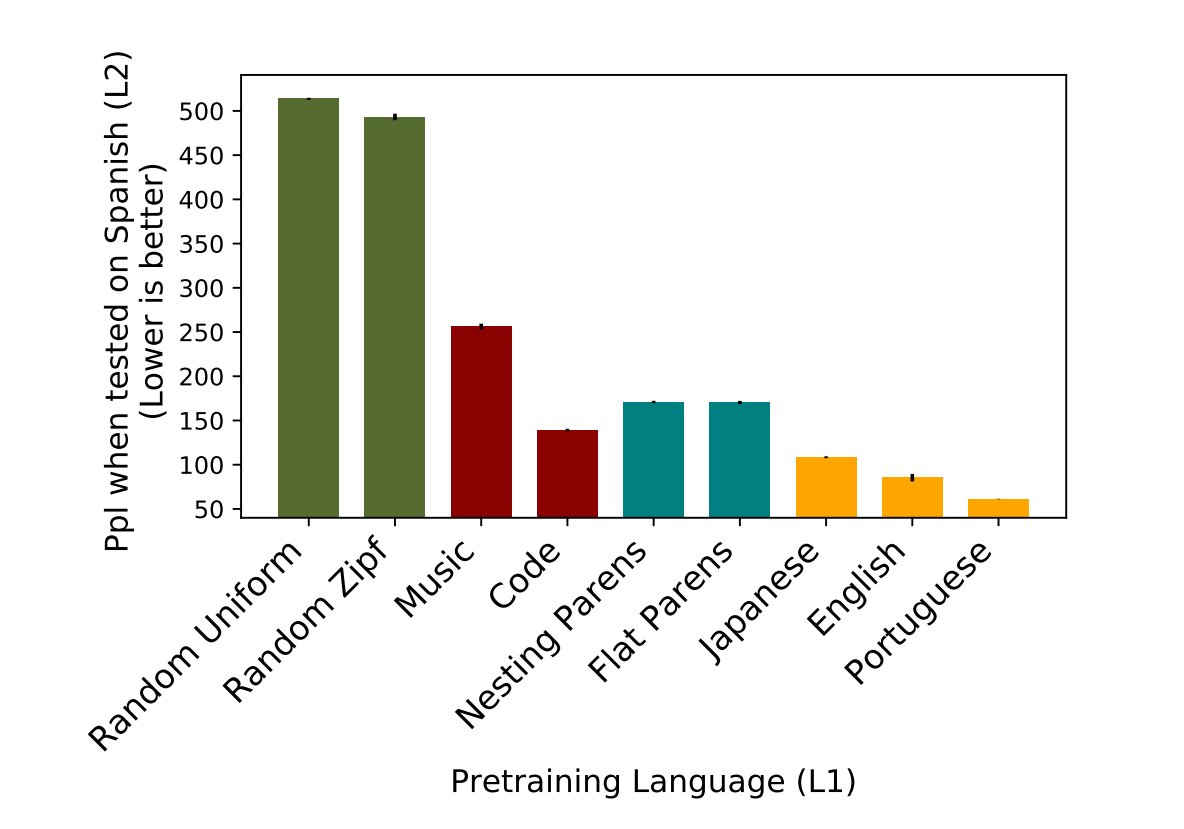
\includegraphics[width=8cm]{img/tilt.png}
		\centering
	\end{figure}

	While making such observations is, without doublt, and important step, more
	data-efficiency advances can be expected if the cause of these observations is
	better understood. Therefore, this work attempts to make a small step in that
	direction and introduces more techniques that can be used to study the
	mechanisms of transfer learning.

	First, as can be seen on the diagram above, different pre-training datasets, even
	if they are all not related to the target task, lead to different final
	performance. It suggests an idea that some languages are intrinsically more complex,
	or perhaps more similar to the target language. To better understand the structure
	of the language space I introduce a new synthethic language by combining ideas
	from the previous work and use it as well as two already existing synthethic datasets
	to pre-train the models. Then I fine-tune them to English using three
	different levels of fine-tuning and observe how the performance depends on the
	language and the allowed flexibility of fine-tuning. From theoretical side, I
	provide an algorithm which might be used by the models trained on this
	datasets and discuss the implications for the difficulty of these languages
	and their effect on model parameters during pre-training.

	Second, as one of the settings for transfer learning involves fine-tuning only
	embeddings, they are the natural target for investigation. I explore the structure
	of the learned embeddings, namely, the spectrum of their singular values which
	is a way to understand the effective dimensionality of the data, and the
	performance of KMeans clustering on them with different number of clusters
	which is a way to check how uniformly the embeddings are distributed. To check
	what information is contained in the embeddings I train linear probes to predict
	certain features of the words given their embeddings. Linear probes are a
	popular interpretability technique, but to the best of my knowledge they have not
	been used in this context, i.e. to study the embeddings of models pre-trained on
	different datasets and fine-tuned to the same task.

	Finally, I evaluate the performance of these models in natural language
	understanding. As existing NLU datasets such as GLUE \cite{wang2018glue} and MMLU
	\cite{hendrycks2020measuring} are designed for more capable models, I use GPT-4
	\cite{openai2023gpt4} to generate a simplar benchmark consisting of 12 diverse
	subtasks.

	\section{Background and motivation}

	\subsection{Role of pre-training}
	One way to understand pre-training of language models is that we transfer some
	linguistic knowledge from a task wich lots of data available to a downstream task
	\cite{han2021pre}. But recent findings suggest that it is not the only
	relevant effect, and sometimes even not the most important one.

	\citet{papadimitriou2020learning} pre-trained LSTM \cite{hochreiter1997long}
	on structured but not linguistic data, such as MIDI music, Java code, and two synthetic
	datasets of parentheses. They observed that adapting such model to Spanish by
	fine-tuning only its input and output embeddings gives better perplexity than
	when starting from randomly initialized model. Their findings and the experiment
	setup established a framework which was used in later works and in this one as
	well. I also use synthethic languages introduced in this work, they will be described
	in details in the section about synthethic languages.

	\citet{ri2022pretraining} improved on these results by replacing LSTM with
	Transformer and by changing the synthethic languages. Both improvements are used
	in this work as well. \citet{papadimitriou2023injecting} used GPT-2 \cite{radford2019language},
	and I copy hyperparameter choices for datasets from them. \citet{chiang2022transferability}
	introduce a family of Shuffle languages, which I use to create a new synthethic
	language. \citet{artetxe2019cross} used a similar technique to combine a task-specific
	corpus in English with a corpus in the target language but not related to the task.

	It also works in the opposite direction, \citet{lu2021pretrained} get performance
	on different modalities comparable to training from scratch by fine-tuning only
	the input and output embeddings of the pre-trained GPT-2. They also try different
	fine-tuning approaches, adapting layer norm parameters and the last
	Transformer block in addition to input and output embeddings.

	An ablation in different direction, \citet{sinha2021masked} find that removing
	all information about word order from the pre-training phase does not affect
	the final performance very much, given a fine-tuning phase with the correct word
	order.

	To demonstrate the importance of pre-training task, \citet{krishna2021does} sample
	the training data from a completely artificial language, which consists of
	random n-grams, and observe that pre-training objectives that require processing
	this information somehow, such as copying sentences in the right order, still improve
	performance of the model on summarization tasks compared to randomly initialized
	version.

	Finally, from the perspective of optimization process, pre-training helps because
	it moves model parameters into a flat basin of the loss landscape. \citet{mehta2021empirical}
	confirm it and suggest as the reason why pre-trained models are less susceptible
	to catastrophic forgetting during fine-tuning. \citet{neyshabur2020being} also
	observe it and also show that models fine-tuned from the same checkpoint stay in
	the same basin.

	\subsection{Internal representations}

	Despite all these surprising findings, language models learn higher-level information
	as well, sometimes research discovers in what form this information is stored
	internally. For example, \citet{gurnee2023language} showed that pre-trained language
	models form quite detailed world models, in terms of both time and space
	representations. Namely, it is possible to extract information about where and
	when an event happened by linear projection from layer 50 activations on the
	corresponding token. \citet{li2022emergent} trained a language model to
	predict Othello moves and found that it represented the state of the board
	internally. \citet{jin2023evidence} demonstrate that language models trained
	on code have representations of program states and that quality of this
	representations is highly correlated with their ability to generate correct
	programs.

	Another surprising finding is that language models tend to learn linear
	representations even when they are not explicitly directed to do so. A well-known
	example is Word2vec \cite{mikolov2013efficient}, which showed that applying
	vector arithmetic to word embeddings produces meaningful results. A more recent
	example in this direction, \citet{turner2023activation} found that same trick works
	for GPT-2 activations. \citet{nanda2023othello} showed that Othello-GPT actually
	has linear world model, in \cite{jin2023evidence} the representations are
	linear as well.

	\subsection{Educational value of data}

	As discussed in the introduction, right choice of pre-training data can
	greatly increase the ration of performance metrics to training costs. Here I describe
	the related works in more details.

	\citet{huebner2021babyberta} noted the discrepancy between the large amount of
	data used to train RoBERTa \cite{liu2019roberta} and the amount of data a
	typical child consumes by the time they acquire a basic understanding of
	language grammar. To train BabyBERTa they used language acquisition data, i.e.
	the kind of data which is available to children, and avoided having the model
	predict unmasked tokens, as it was doine in RoBERTa. As the result, the model achieved
	comparable grammatical knowledge with $15times$ less parameters and $6000times$
	less words.

	\citet{eldan2023tinystories} had a similar setting, but with GPT-style instead
	of BERT-style model, and using generated dataset of stories for children
	instead of recordings of casual speech directed to children. They produced a series
	of TinyStories models with parameter count ranging from 1M to 33M, and even
	the smallest model is capable of generating mostly coherent and grammatically
	correct English stories, although with limited vocabulary and knowledge about the
	world. I use their 8M model for all my experiments, as it is expressive enough
	to learn all the tasks used and at the same time is very affordable to train.

	\citet{gunasekar2023textbooks} and \citet{li2023textbooks} scale this up to 1.3B
	models and to new domains. In the first part they find and generate textbook quality
	data to teach programming skills to the model, and the resulting model
	outperforms much larger ones, up to 16B parameters. In the second part they
	focus on natural language reasoning and generate synthethic lessons on diverse
	range of topics related to world knowledge and common sense. Again, it leads
	to significant reduction in model size, as their 1.3B model outperforms 7B
	models on multi-step reasoning benchmarks and matches them on language
	understanding.

	\subsection{Data-driven inductive bias}

	Past data alone is almost never enough to predict unseen data, as doing so
	requires some assumptions about how they are related. Such assumptions are called
	inductive bias. For example, under assumption that the observed samples are generated
	as the ground truth plus some independent noise, we will predict that the
	future samples will be similar to the average. But the same data might lead us
	to entirely different predictions if we assume that the values tend to grow exponentially
	over time, with an unknown growth rate. The term inductive bias refers to such
	set of assumptions and describes in which way the model tends to generalize.

	A useful inductive bias can be instilled into the model by pre-training on data
	that demonstrates it. \citet{mccoy2020universal} use pre-training on natural languages
	with certain properties by model-agnostic meta-learning \cite{finn2017model} to
	find which biases are needed to quickly acquire these languages. \citet{wu2021lime}
	design synthetic datasets requiring deduction, induction and abduction and pre-train
	on them to extract inductive bias for general mathematical reasoning. \citet{lindemann2023injecting}
	pre-train models to simulate finite state transducers given their description
	and achieve better generalization in NLP tasks with similar structure.

	\subsection{Open questions}

	As mentined above, there were many works that studied transfer learning from
	artificial datasets to natural language, for variety of model architectures,
	datasets and fine-tuning methods. However, they all report only superficial
	metrics, like losses and perplexities. To shed light on what actually happens
	during such transfer, in this work I use diverse analysis techniques to get richer
	observations of this process and as a result, hopefully, get deeper insights.
	In particular, I use the following methods:
	\begin{itemize}
		\item Compare the complexity of synthethic languages by training a model on one
			language and then fine-tuning to another.

		\item To get more feedback from these experiments, fine-tuning is done in
			several stages, each one allowing more complexity to be learned.

		\item Study the structure of the embedding space, in terms of the singular
			values of correlation matrix and by running KMeans algorithm on it with
			different number of clusters.

		\item Consider an algorithm that can be learned by the model in order to model
			the datasets used and what it implies about their complexity.

		\item Train linear probes to predict grammatical features of the words represented
			by tokens and their frequency, thus showing what information might be
			contained in the embeddings.

		\item Introduce a new natural languge understanding dataset tailored for less
			capable models which benchmarks the model performance on 12 diverse subtasks.
	\end{itemize}
	\section{Experiments}

	\subsection{Synthethic languages}
	Following hyperparameter choices from \cite{papadimitriou2023injecting}, for
	each of the languages descrbed below I use sequence length of $512$, vocabulary
	size of $500$, and generate $2 \cdot 10^{6}$ sequences so the total size of
	the dataset is approximately $10^{9}$ tokens in each case.

	\subsubsection{\texttt{nested}}
	The predcessor of this dataset was introduced in
	\cite{papadimitriou2020learning}. They used stack-based grammar to generate sequences,
	where each token occurs twice and two pairs of tokens either do not intersect
	or one is nested in another. In other words, balanced bracket sequence with
	multiple types of brackets.

	\cite{ri2022pretraining} suggested to use different tokens for opening and
	closing brackets, and found improved performance. I chose to implement this
	version, so there are $250$ tokens for open brackets and $250$ tokens for closing
	ones.

	Regarding the sampling algorithm for this language, tokens are generated
	sequentially and on each step a random decision is made whether to open a new
	bracket or to close an existing one. If the stack of open brackets is empty or
	there is not enough space before the end of sequence, there is only one option.
	In other cases an openning bracket is chosen with probability $0.4$ and then the
	type of bracket is sampled uniformly.

	Generation algorithm in Python:
	\begin{verbatim}
def nested_dependencies_sequence(
    seq_len: Even,
    vocab_size: Even,
    tokenizer: PreTrainedTokenizerFast,
) -> str:
    p_open = 0.4
    open_types: deque[int] = deque()
    data = [0] * seq_len
    for i in range(seq_len):
        should_open = t.rand(size=()) < p_open
        must_open = not open_types
        must_close = len(open_types) == seq_len - i
        if (should_open or must_open) and not must_close:
            tp = int(t.randint(low=0, high=vocab_size // 2, size=()))
            data[i] = 2 * tp
            open_types.append(tp)
        else:
            tp = open_types.pop()
            data[i] = 2 * tp + 1
    return tokenizer.decode(data)
\end{verbatim}
	Example word from it:

	\verb|<237 237> <249 249> <24 24> <162 162> <175 <211 <59 59> 211> 175> <233 233> <6 6>|

	\subsubsection{\texttt{flat}}
	This language is similar to the previous one and was introduced and enhanced in
	the same works. The only difference is that the nesting property can be
	violated.

	In terms of sampling it means that when a bracket should be closed, now there is
	more than one possibility. I select the bracket to close uniformly from all
	currently open ones.

	Generation algorithm in Python: \begin{verbatim}
def flat_dependencies_sequence(
    seq_len: Even,
    vocab_size: Even,
    tokenizer: PreTrainedTokenizerFast,
) -> str:
    p_open = 0.4
    open_types: list[int] = []
    data = [0] * seq_len
    for i in range(seq_len):
        should_open = t.rand(size=()) < p_open
        must_open = not open_types
        must_close = len(open_types) == seq_len - i
        if (should_open or must_open) and not must_close:
            tp = int(t.randint(low=0, high=vocab_size // 2, size=()))
            data[i] = 2 * tp
            open_types.append(tp)
        else:
            pos = int(t.randint(low=0, high=len(open_types), size=()))
            tp = open_types.pop(pos)
            data[i] = 2 * tp + 1
    return tokenizer.decode(data)
\end{verbatim}

	Example world: \verb|<216 216> <148 <46 148> 46> <65 <232 65> <225 <199 232> <123 225> <28 123> <106 106>|

	\subsubsection{\texttt{flat\_shuffle}}
	The languages described above are each based on a single rule. While such simplicity
	certainly makes analysis easier, I hypothesized that adding more complexity
	into the data can improve model performance.

	I decided to use an idea of `Shuffle` languages from
	\cite{chiang2022transferability} as an extra pattern, because it was orthogonal
	to the bracket balancing essence of the previous datasets. The combined
	dataset is based on \texttt{flat}, but each consecutive group of $16$ tokens
	has a range of $8$ bracket types assigned to it, and all brackets on this segment
	are sampled only from these types. That is, each such group is a permutation of
	the corresponding brackets.

	It adds two interesting dynamics to the task of next token prediction. When in
	the middle of the sequence, the model needs to look at previous tokens to guess
	the range of bracket types. And when close to the end of permutation, the model
	can guess increasingly more accurately by remembering which tokens were already
	used. In particular, the last token in each permutation can be predicted with certainty.
	Surprisingly, even small Transformer models were able to capture this pattern and
	indeed predicted the last token with close to zero loss.

	Generation algorithm in Python:

	\begin{verbatim}
def flat\_shuffle_sequence(
    seq_len: Even,
    group_len: int,
    vocab_size: Even,
    tokenizer: PreTrainedTokenizerFast,
) -> str:
    p_open = 0.4
    open_types: list[int] = []
    data = [0] * seq_len
    shuffled_range: list[int] = []
    for i in range(seq_len):
        if not shuffled_range:
            range_start = int(t.randint(0, vocab_size // 2 - group_len, size=()))
            range_tensor = t.arange(range_start, range_start + group_len)
            shuffled_range = range_tensor[t.randperm(group_len)].tolist()
        should_open = t.rand(size=()) < p_open
        must_open = not open_types
        must_close = len(open_types) == seq_len - i
        if (should_open or must_open) and not must_close:
            tp = shuffled_range.pop()
            data[i] = 2 * tp
            open_types.append(tp)
        else:
            pos = int(t.randint(low=0, high=len(open_types), size=()))
            tp = open_types.pop(pos)
            data[i] = 2 * tp + 1
    return tokenizer.decode(data)
\end{verbatim}

	Example word: \verb|<58 <61 61> <54 58> 54> <57 57> <55 <56 <60 56> <59 55> 60> 59> <120 <121 120> 121> <125 <124 124> 125>|

	\subsection{Hierarchy of language complexity}

	\subsubsection{Methodology}

	Some languages, both synthethic and naturals, are more complex than others. For
	example, it is much easier to understand the concept of balanced bracket
	sequences than to learn Chinese. Moreover, some languges can be understood
	easier if the learned already knows another language, e.g. humans need less
	effort to switch to a language from the same language family and large
	language models can be fine-tuned to a similar downstream task by using much
	less data than was used for their pre-training. But how to formalize this notion
	of complexity and similary, and how to measure it?

	One approach is the Chomsky hierarchy of languages \cite{chomsky1956three}. It
	formally defines several classes of grammars, each one strictly more general
	than the previous one, and the properties of these classes are very well understood.
	It is very useful as a high-level formalization of language complexity, which can
	show that one language is qualitatively more complex than another. For example,
	\texttt{nested} is a context-free language, while \texttt{flat} is context-dependent.
	But for languages from the same class we need some other tool to find more fine-grained
	differences.

	As the main topic of this work is transfer learning, a natural approach is to
	use transfer learning metrics to estimate both the complexity and similarity
	of languages. For a given language pair I pre-train a language model on the first
	language and then fine-tune it on the second language, in several stages. On the
	first stage I freeze all model parameters except for embeddings and unembeddings,
	so that the internal computations are preserved as much as possible. On the second
	stage the affine parameters of LayerNorms are also fine-tuned, which allows
	the model to re-scale the intermediate activations and thus focus on different
	features. Finally, the last Transformer block is fine-tuned, which allows some
	amount of arbitrary task-specific computation. I don't consider fine-tuning
	all parameters, because in the limit it can reach the same performance as the model
	trained on the second language from scratch and it will be not informative.

	An important obseration is that transfer learning between languages is not symmetric,
	and it allows to estimate both (relative) complexity and similarity of two
	languages. If languages are similar, fine-tuning should go well in both
	directions, so we can take average difficulty of fine-tuning from both directions
	as a measure of similarity. And if one language is more complex than another, at
	least in a sense of having strictly more patterns, one would expect fine-tuning
	to run much easier from the hard language to the easy one, so comparison of two
	directions allows us to reason about hierarchy of languages in terms of complexity.

	This procedure is not completely formalized, in particular, I don't have a principled
	way to measure the "difficulty" of fine-tuning. An approach that seems
	reasonable is to look at the first stage of fine-tuning which is enough to get
	the performance close to the performance of the model pre-trained on the
	second language.

	\subsubsection{Results}
	For all experiments I used TinyStories-8M model \cite{eldan2023tinystories}. For
	pre-training I was waiting till convergence close to theoretical lower bounds of
	loss, or just long stagnation, which took $40$K to $100$K steps. Batch size
	was $8$ and sequence length was $512$ tokens, so I used $160$M to $400$M tokens
	for pre-training. For fine-tuning, at each stage I used a fixed amount of 12500
	steps, batch size was again $8$ and sequence length was $512$ for bracket
	datasets and $128$ for English (TinyStories), which means $51$M and $13$M tokens
	correspondingly. Learning rate was $10^{(}-3)$ for the pre-training and
	$[10^{(}-2), 2 dot 10^{(}-2), 10^{(}-3)]$ for the three stages of fine-tuning.

	The table below presents the results of fine-tuning in both directions on
	certain pairs of languages. Columns "L2 ..." describe fine-tuning on the second
	language after pre-training on the first one, "L2 full" is the performance of
	the model trained on the second language from scratch. Columns "L1 ..." and "L1
	full" are symmetrical, for fine-tuning on the first language. "E", "L" and "T"
	mean what layers were fine-tuned and stand for embeddings, LayerNorms and (the
	last) Transformer block. I use the absolute difference of 0.2 nats per token
	as a threshold for "close performance".

	\begin{table}[ht]
		\centering
		\begin{tabular}{|p{45pt}|p{45pt}|p{20pt}|p{20pt}|p{20pt}|p{20pt}|p{20pt}|p{20pt}|p{20pt}|p{20pt}|}
			\hline
			\textbf{L1}   & \textbf{L2}   & \textbf{L2 E} & \textbf{L2 EL} & \textbf{L2 ELT} & \textbf{L2 full} & \textbf{L1 E} & \textbf{L1 EL} & \textbf{L1 ELT} & \textbf{L1 full} \\
			\hline
			nested        & flat          & 4.41          & 4.14           & 4.08            & 3.78             & 3.47          & 3.34           & 3.34            & 3.32             \\
			\hline
			flat          & flat\_shuffle & 2.46          & 2.36           & 2.15            & 2.00             & 3.82          & 3.80           & 3.76            & 3.78             \\
			\hline
			flat\_shuffle & English       & 2.42          & 2.30           & 2.00            & 1.19             & 2.77          & 2.62           & 2.11            & 2.00             \\
			\hline
			nested        & English       & 2.82          & 2.65           & 2.37            & 1.19             & 3.83          & 3.46           & 3.32            & 3.32             \\
			\hline
			flat          & English       & 2.74          & 2.56           & 2.35            & 1.19             & 4.28          & 4.16           & 3.76            & 3.78             \\
			\hline
		\end{tabular}
		% \caption{}
		% \label{}
	\end{table}

	The first two rows show that \texttt{flat} is more complex than \texttt{nested}
	and \texttt{flat\_shuffle} is more complex than \texttt{flat}, in a sense of
	being more general, because fine-tuning in the direction \texttt{flat\_shuffle}
	$\to$ \texttt{flat} $\to$ \texttt{nested} achieves good performance simply by
	replacing the embeddings. The remaining measurements showo that English is more
	complex than all synthetic languages used here, but it is also quite different,
	as the models needs more flexibility to adapt from English to e.g. \texttt{flat}
	and \texttt{flat\_shuffle}.

	\subsubsection{Mechanistic interpretability}
	As discussed before, \texttt{nested} is a context-free language while \texttt{flat}
	is context-dependent. However, the fact that they lie in different classes does
	not explain, for example, why the second one leads to better structured embedding
	space. So, to have a better chance of understanding the complexity of language
	and its structure, reasoning in terms of abstract classes of languages and
	other high-level generalizations is not enough, and one should understand the actual
	algorithm implemented by the language model trained on it.

	My first step in this investigation was to check the importance of different layers
	on the end result. The model considered was the one trained on \texttt{nested},
	because it is both simple and very structured language, so it is easy to detect
	whether the model works or not. I took the average loss on several prompts as
	a metric and then tried zeroing out every parameter tensor in the model one at
	a time, comparing their impact on the performance. The result was that the
	most impactful layers are the first and the last one, and also embeddings and unembeddings,
	but the middle ones still had a nontrivial impact. In other words, I wasn't
	able to reduce the model to a simpler one.

	As a less agressive technique, I tried replacing each layer by its low-rank approximation.
	Again, the middle layers were the easiest to compress, rank $4$ (out of $d_{"}m
	odel" = 256$) approximation of layers $2 - 5$ still recovered most of the
	performance. But even for rank $4$ matrices it is not trivial to understand what
	algorithm is implemented by them, so this approach was not very productive as
	well.

	Then I tested the model on prompts like \verb|<1 <2 <3 ... <n n> ... 3> 2> 1>|
	and looked for the maximum $n$ for which the next token has the highest
	predicted probability at every position with a closing bracket. I found that the
	maximum $n$ was $16$, which combined with the fact that the model has $8$
	layers allows to reject the hypothesis that each layer increases maximum
	nesting depth by $1$. At the same time, the model clearly had not learnt the
	general algorithm, otherwise it would work for any $n$, or at least much
	larger ones.

	These observations inspired me to think about algorithms that use arithmetic
	in vector spaces to approximate a stack. In particular, I made the following
	algorithm, which predicts the token on top of the stack in a vectorized fashion:

	\begin{verbatim}
import torch as t

t.manual_seed(0)
n_types = 24
dim = 16
factor = 2.0

type_embedding_matrix = t.randn((n_types, dim))
type_embedding_matrix /= type_embedding_matrix.norm(dim=1, keepdim=True)

n_pairs = 16
is_open = t.tensor([1] * n_pairs + [0] * n_pairs + [1] * n_pairs + [0] * n_pairs)
bracket_type = t.tensor(
    list(range(n_pairs))
    + list(range(n_pairs - 1, -1, -1))
    + list(range(n_pairs))
    + list(range(n_pairs - 1, -1, -1))
)

elevation = t.cumsum(2 * is_open - 1, dim=0) - is_open
weight = t.pow(factor, elevation)
signed_weight = (2 * is_open - 1) * weight
type_embeddings = type_embedding_matrix[bracket_type]
weighted_embeddings = signed_weight.unsqueeze(-1) * type_embeddings
prefix_sums = t.cumsum(weighted_embeddings, dim=0)
denominator = t.pow(factor, -(elevation + is_open))
normalized = prefix_sums * denominator.unsqueeze(-1)
logits = normalized @ type_embedding_matrix.T
\end{verbatim}

	The idea is that each type of bracket has a direction associated with it, and stack
	is a single vector, for which the distribution of the possible element "on top
	of the stack" is given by dot products with the type directions, optionally normalized
	by the sum of the weights. To put something on top, I just add the corresponding
	direction with large enough weight so that it dominates everything that was accumulated
	in the stack before. And to pop from the stack, I subtract the same direction.

	The algorithm produces accurate preditions, putting most of the probability
	mass into the correct token:

	\begin{figure}[t]
		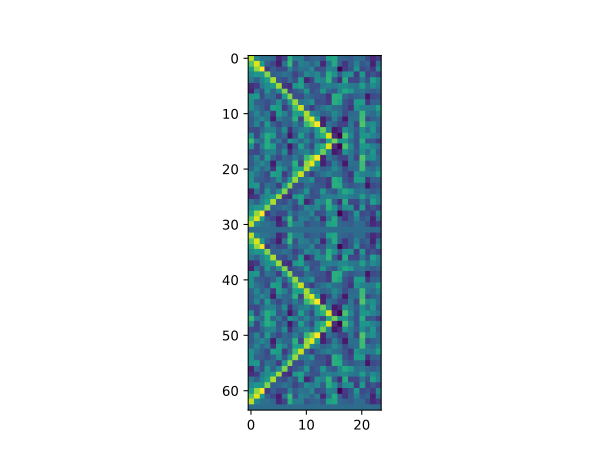
\includegraphics[width=8cm]{img/mech.png}
		\centering
	\end{figure}

	Checking in what way what the language model actually does corresponds to this
	algorithm remains an open question, however it seems plausible that it
	implements at least an approximation of this, e.g. exponentiation is a hard
	operation for a language model so it might instead learn a piecewise-linear
	function to approximate $2^{x}$. There is evidence that the model does not exactly
	this, as the similar plot of log-probabilities of predictions from the model
	looks different, especially the fist half:

	\begin{figure}[t]
		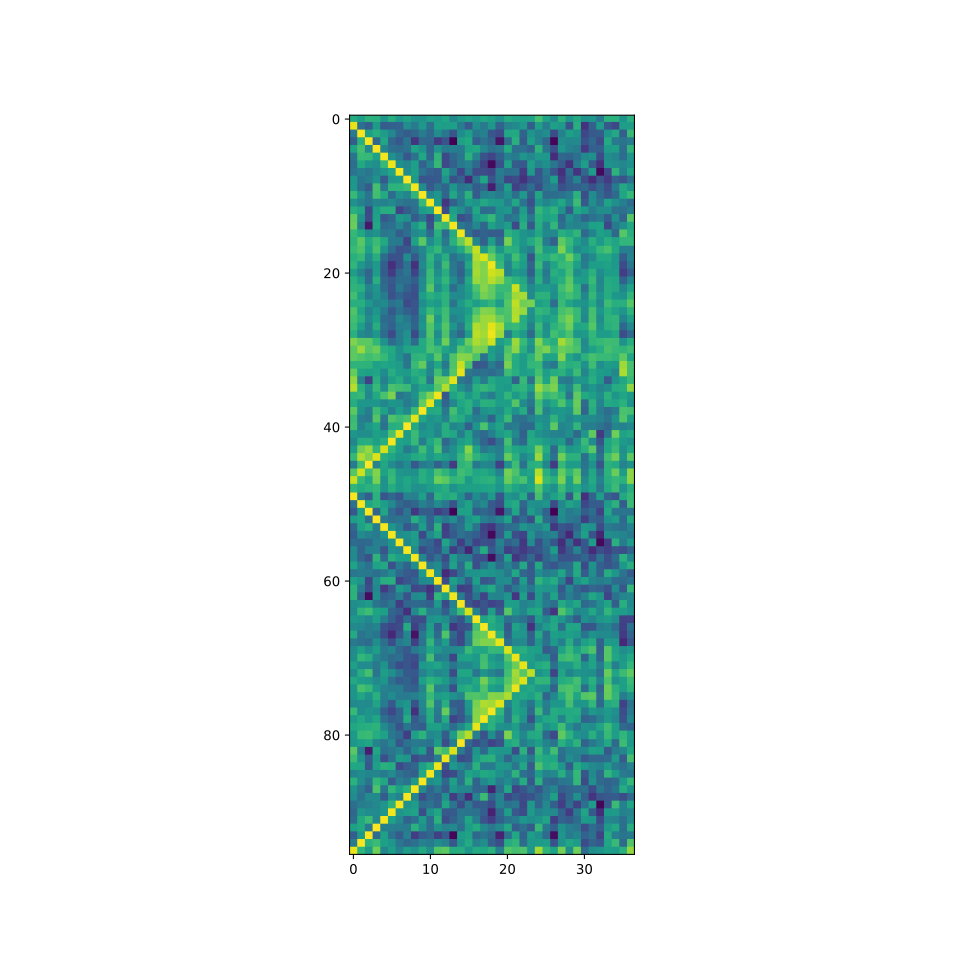
\includegraphics[width=8cm]{img/observed.png}
		\centering
	\end{figure}

	Note that the algorithm can be trivially extended to \texttt{flat} language,
	by removing the exponentiation part --- now the "stack" is simply a sum of the
	embeddings of tokens in it.

	This provides a partial explanation of the structure of the embedding space. For
	\texttt{nested}, the only important property is that each vector has higher dot
	product with itself than with other vectors, because the embedding of the last
	open bracket will have more weight than all other tokens in the stack and so
	they will not interfere with eah other. But for \texttt{flat} the model needs
	access not only to the top of the stack, but to all the tokens in it, which
	means that arbitrary linear combination of the embeddings should be uniquely
	decodable. This requires the embeddings to be orthogonal. However, this does not
	explain why the embeddings during fine-tuning will get the same structure as during
	pre-training. To check if it is the case for pre-training, for all four models
	I measured whether their embedding vectors have the same, or close, norm, and
	whether they are close to orthogonal. The results are shown in the table below.
	Covariance means the average dot product of two different embedding vectors, and
	variance means the average squared norm of an embedding vector.

	\begin{table}[ht]
		\centering
		\begin{tabular}{|p{60pt}|p{40pt}|p{40pt}|p{40pt}|p{40pt}|}
			\hline
			           & \textbf{nested} & \textbf{flat} & \textbf{shuffle} & \textbf{scratch} \\
			\hline
			norm mean  & 3.60            & 3.70          & 4.05             & 0.79             \\
			\hline
			norm std   & 1.31            & 1.13          & 1.23             & 0.29             \\
			\hline
			covariance & 0.65            & 0.19          & 0.06             & 0.16             \\
			\hline
			variance   & 14.68           & 14.97         & 17.94            & 0.72             \\
			\hline
		\end{tabular}
		% \caption{}
		% \label{}
	\end{table}

	The ratio of the covariance to the variance is $4$ times smaller for \texttt{flat}
	and even smaller for `shuffle`, which supports the explanation above.

	\subsection{Word-level information}
	There are non-trivial performance gains in all language pairs from simply
	tuning the embeddings, so in this section I am going to analyze the structure of
	the embedding space and what information about words can be extracted from the
	embeddings.

	\subsubsection{Dimensionality and clusters}

	The embedding dimension of the model used is $d = 256$, and human intuition,
	as well as many visualization techniques, works poorly for $256$-dimensional vectors,
	so I employ two quantitative approaches.

	First, for a $n \times d$ matrix of embeddings $E$, I consider its singular
	values (after zeroing out the mean of each column), or equivalently, the
	spectrum of the covariation matrix $A = E^{T} E$. The motivation behind this is
	that if all embeddings were contained in a $k$-dimensional subpace, and $E$
	had a rank $k$, then only $k$ of the singular values would be nonzero. For
	real data it is not the case, all singular values are nonzero due, but still
	some directions have much larger variance then others and the model is more
	likely to use features corresponding to those dimensions.

	As we see in the figure below, in models pre-trained on synthetic datasets the
	spectrum is dominated by the first few dimensions. In particular, before the fine-tuning,
	most of the interesting information about brackets is described by two axes: open-close
	and low-to-high bracket type id. And while they learn more diverse features
	during fine-tuning on English, as described in the next sections, they still
	don't use the embedding space very efficiently. But the interesting observation
	is how the tail of the spectrum behaves for models trained on different datasets:
	spectrum of \texttt{flat} decays to zero slower than the one of \texttt{nested},
	but the shape is similar, while the spectrum of `shuffle` crosses \texttt{flat}
	at some point and behaves more similar to the spectrum of the model trained on
	English from scratch.

	\begin{figure}[t]
		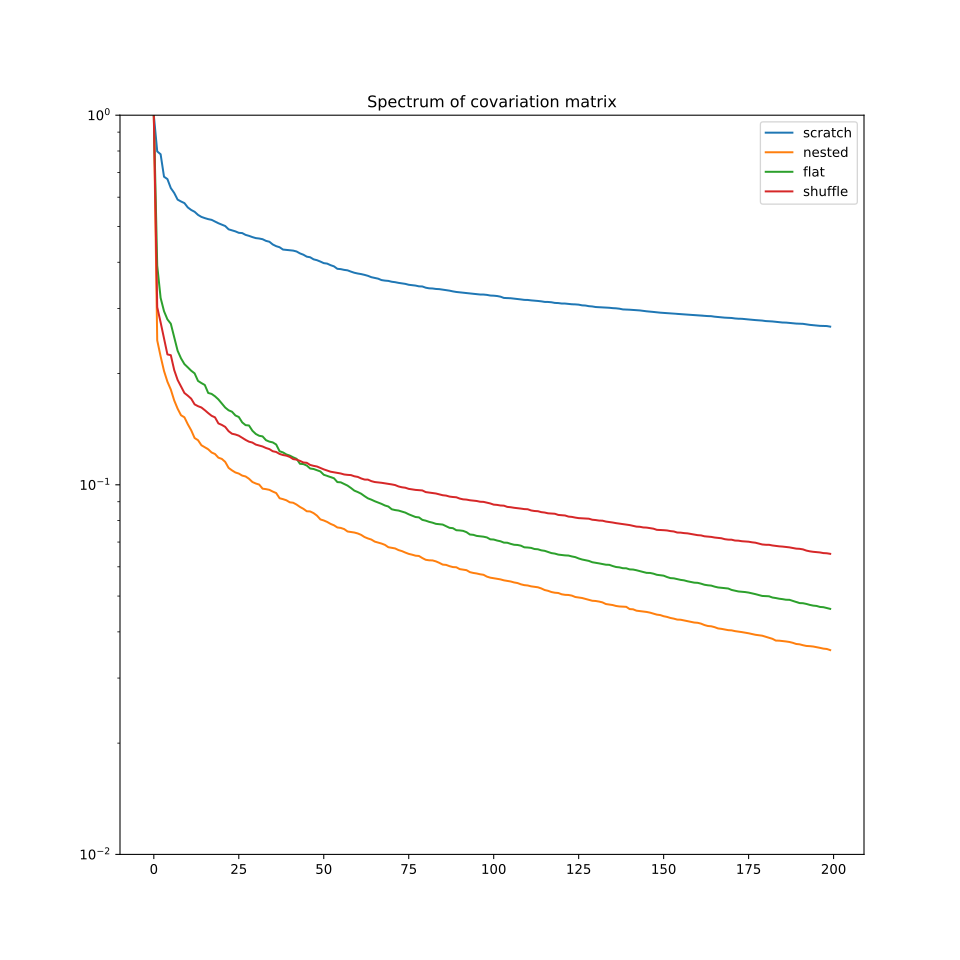
\includegraphics[width=8cm]{img/spectrum.png}
		\centering
	\end{figure}

	Another interesting property is how the embeddings are clustered. To quantify it,
	I run k-means clustering for the embeddings varying the number of clusters and
	compare the plots of unexplained variance (inertia). Again, after pre-training
	on a synthethic language the models have only two clusters: open and close brackets,
	and even after fine-tuning the first few splits explain the majority of
	variance. But looking at the tail behaviour we observe a similar pattern:
	English is followed by \texttt{flat\_shuffle}, then by \texttt{flat} and then by
	\texttt{nested}.

	\begin{figure}[t]
		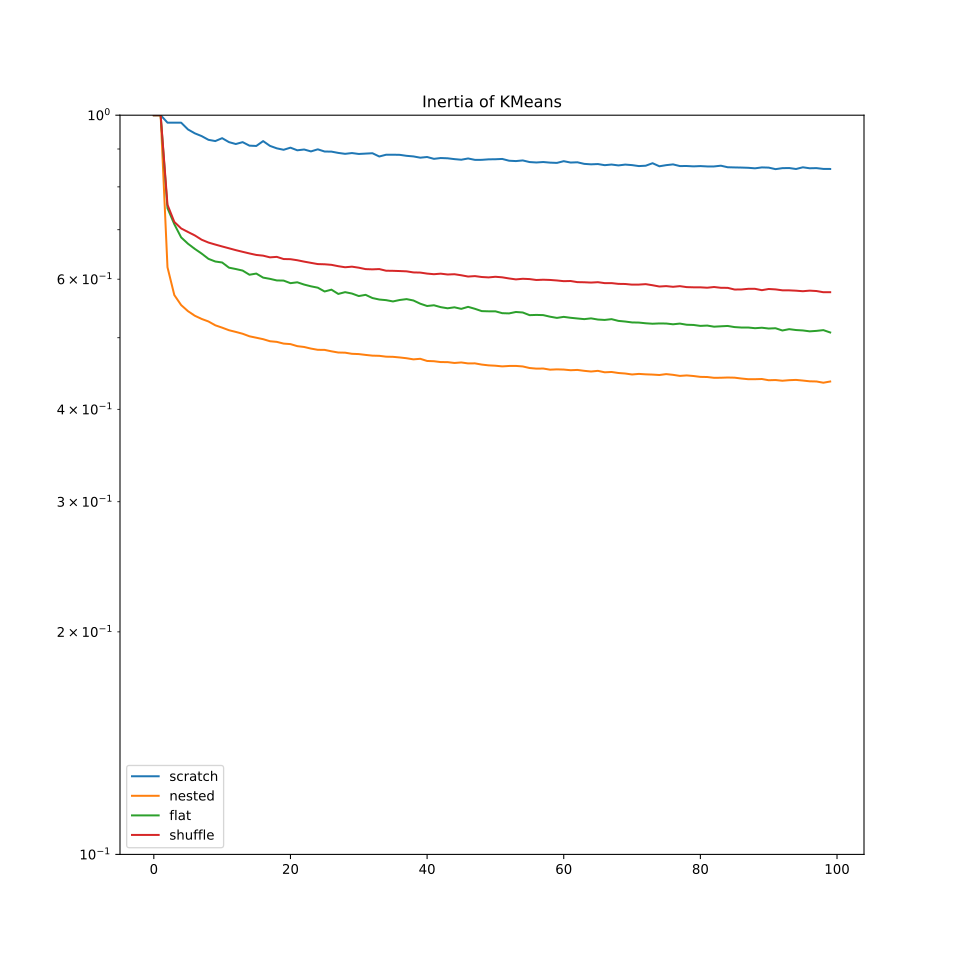
\includegraphics[width=8cm]{img/clusters.png}
		\centering
	\end{figure}

	\subsubsection{Linear probes for word features}

	Now that we know something about the structure of the embedding space, a natural
	question to ask is how this structure is used. In other words, what information
	about a word can one extract from the embedding of the corresponding token.

	Preliminary experiments showed that clusters of features correspond to properties
	like "noun", "3rd person verb", "adjective or adverb", etc. Therefore I decided
	to use part-of-speech tags provided by NLTK library as targets. Initially
	there were more than $30$ unique tags in the dataset, but many of them were very
	rare. After filtering out all tags with less than $200$ occurences the
	following tags remained:
	\begin{itemize}
		\item CD: cardinal digit

		\item IN: preposition or subordinating conjunction

		\item JJ: adjective

		\item NN: singular noun

		\item NNP: proper noun

		\item NNS: plural noun

		\item RB: adverb

		\item VB: base form verb

		\item VBD: past tense verb

		\item VBG: gerund

		\item VBN: past participle
	\end{itemize}

	I added a feature indicating the frequency of the token in the training corpus,
	because typically the direction with the most variance in the embedding space roughly
	corresponded to frequency. And the last feature is whether the token starts
	with a whitespace, as some clusters had disproportionate amount of such tokens.

	For each of the models and each of the features I trained a ridge regression (for
	frequency) or a logistic regression (for all other variables, as they are boolean)
	on $80\%$ of the embeddings and then evaluated their $R^{2}$ score or ROC-AUC
	on the remaining $20\%$.

	\begin{table}[ht]
		\centering
		\begin{tabular}{ |p{60pt} |p{40pt} |p{40pt} |p{40pt} |p{40pt}| }
			\hline
			                 & \textbf{nested} & \textbf{flat} & \textbf{shuffle} & \textbf{scratch} \\
			\hline
			frequency        & 0.84            & 0.85          & 0.85             & 0.93             \\
			\hline
			start\_space     & 0.70            & 0.70          & 0.70             & 0.89             \\
			\hline
			pos\_tag\_CD     & 0.66            & 0.63          & 0.63             & 0.80             \\
			\hline
			pos\_tag\_IN     & 0.76            & 0.79          & 0.71             & 0.87             \\
			\hline
			pos\_tag\_JJ     & 0.60            & 0.58          & 0.60             & 0.73             \\
			\hline
			pos\_tag\_NN     & 0.63            & 0.62          & 0.63             & 0.76             \\
			\hline
			pos\_tag\_NNP    & 0.64            & 0.65          & 0.63             & 0.79             \\
			\hline
			pos\_tag\_NNS    & 0.67            & 0.67          & 0.68             & 0.84             \\
			\hline
			pos\_tag\_RB     & 0.69            & 0.63          & 0.64             & 0.84             \\
			\hline
			pos\_tag\_VB     & 0.71            & 0.69          & 0.68             & 0.79             \\
			\hline
			pos\_tag\_VBD    & 0.75            & 0.71          & 0.67             & 0.89             \\
			\hline
			pos\_tag\_VBG    & 0.71            & 0.70          & 0.73             & 0.89             \\
			\hline
			pos\_tag\_VBN    & 0.72            & 0.68          & 0.72             & 0.87             \\
			\hline
			\textbf{Average} & 0.70            & 0.68          & 0.68             & 0.84             \\
			\hline
		\end{tabular}
		% \caption{}
		% \label{}
	\end{table}

	All probes in for all models perform better than random, so every model learns
	at least something related to this features. The embeddings of the model trained
	on English from scratch predictably outperformed the others, but the quality
	of other embeddings turned out to be on average the same. Perhpaps the difference
	in effective dimension between the models is used not for this relatively simple
	single word features, but for word meanings, sentence structure and so on.

	\subsubsection{Cloze tests}

	To assess how good the models are in understanding language in general a
	different benchmark is needed. As the models studied are too small for reliable
	question answering, reasoning and other high-level cognitive skills, the test should
	be as simple as possible, ideally just measuring perplexity on some texts. There
	are several already existing datasets for natural language understanding, such
	as GLUE \cite{wang2018glue} and MMLU \cite{hendrycks2020measuring}, and they have
	many diverse subtasks, but they focus on more complex tasks.

	Instead, I used GPT-4 \cite{openai2023gpt4} to generate a set of cloze infilling
	questions in simple English. There are the following $12$ subtasks, each with $1
	0$ cloze questions:
	\begin{itemize}
		\item Synonyms and antonyms.

		\item Logical relations.

		\item Subject-verb agreement.

		\item Prepositions.

		\item Conjunctions.

		\item Temporal understanding.

		\item Spatial understanding.

		\item Quantitative reasoning.

		\item Emotions.

		\item Narrative understanding.

		\item Ethics.
	\end{itemize}

	Each cloze question consists of a prompt with a cloze marker, a correct answer
	and an incorrect answer. For each question the difference between log-probabilities
	of the correct and incorrect answers is measured and then averaged across each
	subtask.

	An example from the temporal understanding subtask:

	\texttt{[ "She ate breakfast \# she went to school", "before", "after", ] }

	For each of the synthetic languages I used two models, one where only the fine-tunings
	were adapted to English (E) and another with all three stages (ELT). I compared
	them to the model of the same architecture trained on English from scratch,
	and also to a four times bigger model trained on English from scratch to see
	which metrics can be improved.

	\begin{table}[ht]
		\centering
		\begin{tabular}{|p{90pt}|*{8}{p{33pt}|}}
			\hline
			                        & \textbf{nested ELT} & \textbf{nested E} & \textbf{flat ELT} & \textbf{flat E} & \textbf{shuffle ELT} & \textbf{shuffle E} & \textbf{scratch 8M} & \textbf{scratch 33M} \\
			\hline
			synonyms and antonyms   & 0.18                & 0.24              & 0.13              & 0.22            & 0.25                 & 0.31               & 0.25                & 0.28                 \\
			\hline
			single plural           & 0.15                & 0.08              & 0.50              & 0.19            & 0.33                 & 0.03               & 0.58                & 0.71                 \\
			\hline
			logical relations       & -0.30               & -0.08             & -0.18             & -0.44           & -0.08                & -0.13              & -0.04               & 0.09                 \\
			\hline
			subject verb agreement  & 0.45                & 0.54              & 0.36              & 0.46            & 0.26                 & 0.14               & 0.83                & 0.98                 \\
			\hline
			prepositions            & 0.52                & 0.43              & 0.53              & 0.51            & 0.48                 & 0.40               & 0.94                & 1.12                 \\
			\hline
			conjunctions            & 0.43                & 0.46              & 0.38              & 0.45            & 0.49                 & 0.36               & 0.63                & 0.82                 \\
			\hline
			temporal understanding  & -0.02               & -0.13             & 0.04              & -0.14           & 0.36                 & 0.09               & 0.44                & 0.73                 \\
			\hline
			spatial understanding   & 0.30                & 0.13              & 0.48              & 0.40            & 0.37                 & 0.06               & 0.64                & 0.71                 \\
			\hline
			quantitative reasoning  & 0.00                & -0.06             & -0.01             & -0.14           & -0.04                & -0.14              & -0.04               & -0.06                \\
			\hline
			emotions                & 0.03                & -0.08             & 0.07              & 0.05            & -0.01                & 0.20               & 0.61                & 0.77                 \\
			\hline
			narrative understanding & -0.04               & -0.07             & 0.07              & 0.03            & 0.04                 & 0.04               & 0.17                & 0.27                 \\
			\hline
			ethics                  & 0.17                & 0.32              & 0.22              & 0.34            & 0.30                 & 0.27               & 0.25                & 0.51                 \\
			\hline
			\textbf{Average}        & 0.16                & 0.15              & 0.22              & 0.16            & 0.23                 & 0.14               & 0.44                & 0.58                 \\
			\hline
		\end{tabular}
		\caption{Your table caption here}
		\label{your-label-here}
	\end{table}

	In terms of general trends there are two interesting observations. First, models
	with all three stages of fine-tuning are better, predictably, than their counterparts
	having only the embeddings tuned, but this difference is more pronounced in
	\texttt{flat} and \texttt{flat\_shuffle}. The question why is it so remain open
	for the future work. Second, a familiar pattern appears again, \texttt{nested}
	\textless \texttt{flat} \textless \texttt{flat\_shuffle} \textless `scratch`,
	which proves the superiority of the introduced \texttt{flat\_shuffle} dataset.

	\section{Conclusion}

	A new synthethic language \texttt{flat\_shuffle} was introduced and the model pre-trained
	on it was shown to outperform the models based on the languages from previous work.

	Investigation of the struture of the embeddings leads to a hypothesis that a reason
	behind the superior performance of some synthethic languages is that they require
	more orthogonal embeddings in pre-training task, which causes the intermediate
	layers to be adapted to work with such embeddings, and in turn allows effectively
	using higher dimension subspace of the embedding space during fine-tuning,
	which gives more flexibility. Testing this hypothesis is left for the future work.

	No direct transfer of knowledge or structure was found, instead it seems that
	models are working in reservoir computing style where the computations for an
	unrelated task are adapted to the task at hand in arbitrary ways. At the same time
	it means that the models are not stricty limited by the complexity or structure
	of the original task in transfer learning, and as long as they have enough
	complexity of computations, they can use it to adapt to the new task.

	% \bibliography{refs}
\end{document}
